%%%%%%%%%%%%%%%%%%%%%%%%%%%%%%%%%%%%%%%%%%%%%%%%%%%%%%%%%%%%%%%%%%%%%%%%%%%%%%%%
%2345678901234567890123456789012345678901234567890123456789012345678901234567890
%        1         2         3         4         5         6         7         8

\documentclass[letterpaper, 10 pt, conference]{ieeeconf}  % Comment this line out if you need a4paper

%\documentclass[a4paper, 10pt, conference]{ieeeconf}      % Use this line for a4 paper

\IEEEoverridecommandlockouts                              % This command is only needed if
                                                          % you want to use the \thanks command

\overrideIEEEmargins                                      % Needed to meet printer requirements.

%In case you encounter the following error:
%Error 1010 The PDF file may be corrupt (unable to open PDF file) OR
%Error 1000 An error occurred while parsing a contents stream. Unable to analyze the PDF file.
%This is a known problem with pdfLaTeX conversion filter. The file cannot be opened with acrobat reader
%Please use one of the alternatives below to circumvent this error by uncommenting one or the other
%\pdfobjcompresslevel=0
%\pdfminorversion=4

% See the \addtolength command later in the file to balance the column lengths
% on the last page of the document

% The following packages can be found on http:\\www.ctan.org
%\usepackage[utf8]{inputenc}
\usepackage{amsfonts,amsmath,amssymb}
\usepackage{bm}
\usepackage{float}
\usepackage{graphicx}
\usepackage{color}
%\usepackage[dvipdfmx]{hyperref}
\usepackage{algorithm}
\usepackage{algorithmic}
%\usepackage{txfonts}
%\usepackage{ascmac, here}
\usepackage{listings}
\usepackage{color}
%\usepackage{url}
\usepackage{comment}
\usepackage{cite}
\allowdisplaybreaks[1]

\newtheorem{theorem}{Theorem}
\newtheorem{corollary}{Corollary}
\newtheorem{lemma}{Lemma}
\newtheorem{prop}{Proposition}
\newtheorem{definition}{Definition}

%\theoremstyle{definition}
%\newtheorem{definition}{Definition}[section]

%\theoremstyle{remark}
\newtheorem{remark}{Remark}

\newcommand{\argmax}{\mathop{\rm arg~max}\limits}
\newcommand{\argmin}{\mathop{\rm arg~min}\limits}

\title{\LARGE \bf
Reinforcement Learning of Control Policy for Linear Temporal Logic Specifications Using Limit-Deterministic B\"{u}chi Automata
}


\author{Ryohei Oura, Ami Sakakibara, and Toshimitsu Ushio% <-this % stops a space
\thanks{This work was partially supported by JST-ERATO HASUO Project Grant Number JPMJER1603, Japan, JST-Mirai Program Grant Number JPMJMI18B4, Japan, and JSPS KAKENHI Grant Number JP19J13487, Japan.}% <-this % stops a space
\thanks{The authors are with the Graduate School of Engineering Science, Osaka University, Toyonaka 560-8531, Japan (e-mail: {r-oura, sakakibara}@hopf.sys.es.osaka-u.ac.jp; ushio@sys.es.osaka-u.ac.jp).}%
}



\begin{document}

\maketitle
\thispagestyle{empty}
\pagestyle{empty}

%%%%%%%%%%%%%%%%%%%%%%%%%%%%%%%%%%%%%%%%%%%%%%%%%%%%%%%%%%%%%%%%%%%%%%%%%%%%%%%%
\begin{abstract}

This letter proposes a novel reinforcement learning method for the synthesis of a control policy satisfying a control specification described by a linear temporal logic formula.  We assume that the controlled system is modeled by a Markov decision process (MDP).
We transform the specification to a limit-deterministic B\"{u}chi automaton (LDBA) with several accepting sets that accepts all infinite sequences satisfying the formula.
The LDBA is augmented so that it explicitly records the previous visits to accepting sets.
We take a product of the augmented LDBA and the MDP, based on which we define a reward function.  The agent gets rewards whenever state transitions are in an accepting set that has not been visited for a certain number of steps.
Consequently, sparsity of rewards is relaxed and optimal circulations among the accepting sets are learned. We show that the proposed method can learn an optimal policy when the discount factor is sufficiently close to one.
\end{abstract}

\begin{keywords}
  Reinforcement Learning, Linear Temporal Logic, Limit-Deterministic B\"{u}chi Automata.
\end{keywords}

%%%%%%%%%%%%%%%%%%%%%%%%%%%%%%%%%%%%%%%%%%%%%%%%%%%%%%%%%%%%%%%%%%%%%%%%%%%%%%%%
\section{Introduction}
Temporal logic has been developed in computer engineering as a useful formalism of formal specifications  \cite{BK2008,Clarke2018}.
A merit of temporal logics is its resemblance to natural languages and it has been widely used in several other areas of engineering. Especially, a complicated mission or task in computer-controlled systems such as robots can be described by a temporal logic specification precisely and many synthesis algorithms of a controller or a planner that satisfies the specification have been proposed \cite{KB2008,Gazit2009,WTM2012a,SU2018}.
Linear temporal logic (LTL) is often used as a specification language because of its rich expressiveness.  It can explain many important $\omega$-regular properties such as liveness, safety, and persistence \cite{BK2008}.
It is known that the LTL specification is converted into an $\omega$-automaton such as a nondeterministic B\"{u}chi automaton and a deterministic Rabin automaton \cite{BK2008,Belta2017}.
In the synthesis of a control policy for the LTL specification,  we model a controlled system by a transition system that abstracts its dynamics, construct a product automaton of the transition system and the $\omega$-automaton corresponding to the LTL specification, and compute a winning strategy of a game over the product automaton \cite{Belta2017}.

In general, there are uncertainties in a controlled system and we often use a Markov decision process (MDP) as a finite-state abstraction of the controlled system \cite{Puterman}.
In the case where the probabilities are unknown a priori, we have two approaches to the synthesis of the control policy. One is robust control where we assume that state transition probabilities are in uncertainty sets \cite{WTM2012} while the other is learning using samples \cite{Sadigh2014}.

Reinforcement learning (RL) is a useful approach to learning an optimal policy from sample behaviors of the controlled system \cite{Sutton}.
In RL, we use a reward function that assigns a reward to each transition in the behaviors and evaluate a control policy by the return that is an expected (discounted) sum of the rewards along the behaviors.
Thus, to apply RL to the synthesis of a control policy for the LTL specification, it is an important issue how to introduce the reward function, which depends on the acceptance condition of an $\omega$-automaton converted from the LTL specification.
A reward function based on the acceptance condition of a Rabin automaton was proposed in \cite{Sadigh2014}. It was applied to a control problem where the controller optimizes a given control cost under the LTL constraint \cite{HU2015}.

Recently, a limit-deterministic B\"{u}chi automaton (LDBA) is paid much attention to as an $\omega$-automaton corresponding to the LTL specification \cite{SEJK2016}.
The RL-based approaches to the syntehsis of a control policy using LDBAs have been proposed in \cite{HAK2019,Hahn2019,HKAKPL2019,BWZP2019}.
To deal with the acceptance condition of an LDBA that accepts behaviors visiting all accepting sets infinitely often, the accepting frontier function was introduced in \cite{HAK2019,HKAKPL2019}. The reward function is defined based on the function.
However, the function is memoryless, that is, it does not provide the information of accepting sets that have been visited, which is important to improve learning performance.
In this letter, we propose a novel method to augment an LDBA converted from a given LTL formula.
Then, we define a reward function based on the acceptance condition of the product MDP of the augmented LDBA and the controlled system.
% based on the acceptance condition of the augmented automaton, embedded in the product MDP, which enables us to
As a result, we can learn a dynamic control policy that satisfies the LTL specification.

The rest of the letter is organized as follows.
Section II reviews an MDP, LTL, and automata.
Section III proposed a novel RL-based method for the synthesis of a control policy.
Section IV presents a numerical example for which the previous method cannot learn a control policy but the proposed one can.

\section{Preliminaries}

\subsection{Markov Decision Process}

\begin{definition}
A (labeled) Markov decision process (MDP) is a tuple $M$ = $(S, A, \mathcal{A}, P, s_{init}, AP, L)$, where S is a finite set of states, $A$ is a finite set of actions, $\mathcal{A} : S \rightarrow 2^A$ is a mapping that maps each state to the set of possible actions at the state, $P:S \times S \times A \rightarrow [0,1]$ is a transition probability such that $\sum_{s' \in S} P(s'|s,a) = 1$ for any state $s \in S$ and any action $a \in \mathcal{A}(s) $, $s_{init} \in S$ is the initial state, $AP$ is a finite set of atomic propositions, and $L : S \times A \times S\ \rightarrow\ 2^{AP}$ is a labeling function that assigns a set of atomic propositions to each transition $(s, a, s') \in S \times A \times S$.

In the MDP $M$, an infinite path starting from a state $s_0 \in S$ is defined as a sequence $\rho\ =\ s_0a_0s_1 \ldots\ \in S (A S)^{\omega}$ such that $P(s_{i+1}|s_i, a_i) > 0$ for any $ i \in \mathbb{N}_0$, where $\mathbb{N}_0$ is the set of natural numbers including zero.  A finite path is a finite sequence in $S (A S)^*$. In addition, we sometimes represent $\rho$ as $\rho_{init}$ to emphasize that $\rho$ starts from $s_0 = s_{init}$.
For a path $\rho\ =\ s_0a_0s_1 \ldots$, we define the corresponding labeled path $L(\rho)\ =\ L(s_0,a_0,s_1)L(s_1,a_1,s_2) \ldots \in (2^{AP})^{\omega}$. $InfPath^{M}\ ( \text{resp., }FinPath^{M})$ is defined as the set of infinite (resp., finite) paths starting from $s_0=s_{init}$ in the MDP $M$. For each finite path $\rho$, $last(\rho)$ denotes its last state.
\end{definition}

\begin{definition}
  A policy on an MDP $M$ is defined as a mapping $\pi:FinPath^{M} \times \mathcal{A}(last(\rho)) \rightarrow [0,1]$. A policy $\pi$ is a {\it positional} policy if for any $ \rho \in FinPath^{M}$ and any $ a \in \mathcal{A}(last(\rho))$, it holds that $\pi(\rho, a)=\pi(last(\rho),a)$ and there exists $ a' \in \mathcal{A}(last(\rho))$ such that $\pi(\rho, a) = 1$ if $a=a^{\prime}$, otherwise $\pi(\rho, a) = 0$.
  \begin{comment}
  \begin{align*}
    \pi(\rho, a) =
    \left\{
    \begin{aligned}
      1 &   & &\text{if}\ a=a',\\
      0 &   & &\text{otherwise}.
    \end{aligned}
    \right.
  \end{align*}
\end{comment}
\end{definition}

Let $InfPath^{M}_{\pi}$ (resp., $FinPath^{M}_{\pi}$) be the set of infinite (resp., finite) paths starting from $s_0=s_{init}$ in the MDP $M$ under a policy $\pi$. The behavior of an MDP $M$ under a policy $\pi$ is defined on a probability space $(InfPath^{M}_{\pi}, \mathcal{F}_{InfPath^{M}_{\pi}}, Pr^{M}_{\pi})$. % over the set of infinite paths $InfPath^{M}_{\pi}$ on the MDP $M$ with the policy $\pi$.

A Markov chain induced by an MDP $M$ with a positional policy $\pi$ is a tuple $MC_{\pi} = (S_{\pi},P_{\pi},s_{init},AP,L)$, where $S_{\pi} = S$, $P_{\pi}(s'|s) = P(s'|s,a)$ for $s, s^{\prime} \in S$ and $a \in \mathcal{A}(s)$ such that $\pi(s,a) = 1$.
The state set $S_{\pi}$ of $MC_{\pi}$ can be represented as a disjoint union of a set of transient states $T_{\pi}$ and closed irreducible sets of recurrent states $R^j_{\pi}$ with $j \in \{ 1, \ldots ,h \}$, as $ S_{\pi} = T_{\pi} \sqcup R^1_{\pi} \sqcup \ldots \sqcup R^h_{\pi} $ \cite{ESS}.
In the following, we say a ``recurrent class'' instead of a ``closed irreducible set of recurrent states'' for simplicity.

In an MDP $M$, we define a reward function $R:S \times A \times S \rightarrow \mathbb{R}_{\geq0}$, where $\mathbb{R}_{\geq0}$ is the set of nonnegative real numbers. The function denotes the immediate scalar bounded reward received after the agent performs an action $a$ at a state $s$ and reaches a next state $s'$ as a result.

\begin{definition}
  For a policy $\pi$ on an MDP $M$, any state $s \in S$, and a reward function $R$, we define the expected discounted reward as
  \begin{align*}
    V^{\pi}(s)= \mathbb{E}^{\pi}[\sum_{n=0}^{\infty}\gamma^n R(S_n, A_n, S_{n+1})|S_0 = s],
  \end{align*}
where $\mathbb{E}^{\pi}$ denotes the expected value given that the agent follows the policy $\pi$ from the state $s$ and $\gamma \in [0,1)$ is a discount factor. The function $V^{\pi}(s)$ is often referred to as a state-value function under the policy $\pi$. For any state-action pair $(s,a) \in S \times A$, we define an action-value function $Q^{\pi}(s,a)$ under the policy $\pi$ as follows.
  \begin{align*}
    Q^{\pi}(s,a)= \mathbb{E}^{\pi}[\sum_{n=0}^{\infty}\gamma^n R(S_n, A_n, S_{n+1})|&S_0 = s, A_0 = a].
  \end{align*}
\end{definition}

\begin{definition}
  For any state $s$ in $S$, a policy $\pi^{\ast}$ is optimal if
  \begin{align*}
    \pi^{\ast} \in \argmax_{\pi \in \Pi^{pos}} V^{\pi}(s),
  \end{align*}
where $\Pi^{pos}$ is the set of positional policies over the state set $S$.
\end{definition}

\subsection{Linear Temporal Logic and Automata}

In our proposed method, we use linear temporal logic (LTL) formulas to describe various constraints or properties and to systematically assign corresponding rewards.
%For some complicated constraints, it is hard to assign such a corresponding reward function and to find a policy satisfying an LTL formula by the conventional reward assignments.
LTL formulas are constructed from a set of atomic propositions, Boolean operators, and temporal operators. We use the standard notations for the Boolean operators: $\top$ (true), $\neg$ (negation), and $\land$ (conjunction).
LTL formulas over a set of atomic propositions $AP$ are defined as
\begin{align*}
  \varphi ::=\top\ |\ \alpha \in AP\ |\ \varphi_1 \land \varphi_2\ |\ \neg \varphi\ |\ \text{{\bf X}} \varphi\ |\ \varphi_1 \text{{\bf U}} \varphi_2,
\end{align*}
where $\varphi$, $\varphi_1$, and $\varphi_2$ are LTL formulas.
Additional Boolean operators are defined as $\perp := \neg \top $, $\varphi_1 \lor \varphi_2 := \neg(\neg \varphi_1 \land \neg \varphi)$, and $\varphi_1 \Rightarrow \varphi_2 := \neg \varphi_1 \lor \varphi_2$.
The operators {\bf X} and {\bf U} are called ``next" and ``until", respectively.
Using the operator {\bf U}, we define two temporal operators: (1) {\it eventually}, $\text{{\bf F}} \varphi := \top \text{{\bf U}} \varphi $ and (2) {\it always}, $\text{{\bf G}} \varphi := \neg \text{{\bf F}} \neg \varphi$.

Let $ M $ be an MDP.
For an infinite path $\rho = s_0a_0s_1 \ldots $ of $ M $ with $ s_0 \in S $, let $\rho[i]$ be the $i$-th state of $\rho$ i.e., $\rho[i]=s_i$ and let $\rho[i:]$ be the $i$-th suffix $\rho[i:]=s_ia_is_{i+1} \ldots $.
% let $\rho[:i]$ be the $i$-th prefix $\rho[:i]=s_0 \ldots s_{i-1}a_{i-1}s_i$,and let $\rho[i:j]$ be the finite sequence $\rho[i:j]=s_ia_is_{i+1} \ldots s_{j-1}a_{j-1}s_{j}$.
\begin{definition}
	For an LTL formula $\varphi$, an MDP $M$, and an infinite path $\rho = s_0a_0s_1 \ldots$ of $ M $ with $ s_0 \in S $, the satisfaction relation $M,\rho \models \varphi$ is recursively defined as follows. $M, \rho \models \top$, $M, \rho \models \alpha \in AP \text{ iff } \alpha \in L(s_0,a_0,s_1)$, $M, \rho \models \varphi_1 \land \varphi_2 \text{ iff } M, \rho \models \varphi_1 \land M, \rho \models \varphi_2$, $M, \rho \models \neg \varphi \text{ iff } M, \rho \not\models \varphi$, $ M, \rho \models \text{{\bf X}}\varphi \text{ iff } M, \rho[1:] \models \varphi$, and $M, \rho \models \varphi_1 \text{{\bf U}} \varphi_2 \text{ iff } \exists j \geq 0, \ M, \rho[j:] \models \varphi_2 \land \forall i, 0\leq i < j, \ M, \rho[i:] \models \varphi_1$.
  \begin{comment}
	\begin{alignat}{2}
	& M, \rho \models \top,\nonumber \\
	& M, \rho \models \alpha \in AP &&\Leftrightarrow \alpha \in L(s_0,a_0,s_1),\nonumber \\
	& M, \rho \models \varphi_1 \land \varphi_2 &&\Leftrightarrow M, \rho \models \varphi_1 \land M, \rho \models \varphi_2,\nonumber \\
	& M, \rho \models \neg \varphi &&\Leftrightarrow M, \rho \not\models \varphi,\nonumber \\
	& M, \rho \models \text{{\bf X}}\varphi &&\Leftrightarrow M, \rho[1:] \models \varphi,\nonumber \\
	& M, \rho \models \varphi_1 \text{{\bf U}} \varphi_2 &&\Leftrightarrow \nonumber \\
	& \quad \exists j \geq 0, \ M, \rho[j:] &&\models \varphi_2 \land \forall i, 0\leq i < j, \ M, \rho[i:] \models \varphi_1.\nonumber
	\end{alignat}
\end{comment}
The next operator {\bf X} requires that $\varphi$ is satisfied by the next state suffix of $\rho$. The until operator {\bf U} requires that $\varphi_1$ holds true until $\varphi_2$ becomes true over the path $\rho$.
%Using the operator {\bf U} we can define two temporal operators: (1) {\it eventually}, $\text{{\bf F}} \varphi := \top \text{{\bf U}} \varphi $ and (2) {\it always}, $\text{{\bf G}} \varphi := \neg \text{{\bf F}} \neg \varphi$.
In the following, we write $ \rho \models \varphi $ for simplicity without referring to MDP $ M $.
%For an LTL formula $ \varphi $ over $ AP $,
%we denote by $ \mathcal{L}(\varphi) \subset (2^{AP})^\omega $ the set of all words that satisfy $\varphi$.


For any policy $\pi$, we denote the probability of all paths starting from $s_{init}$ on the MDP $M$ that satisfy an LTL formula $\varphi$ under the policy $\pi$ as
\begin{align*}
Pr^{M}_{\pi}(s_{init} \! \models \varphi) := Pr^{M}_{\pi}(\{ \rho_{init} \! \in \! InfPath^{M}_{\pi} ; \rho_{init} \! \models \varphi \}).
\end{align*}
We say that an LTL formula $\varphi$ is satisfied by a positional policy $\pi$ if
\begin{align*}
Pr^{M}_{\pi}(s_{init} \models \varphi) > 0.
\end{align*}



\label{def5}
\end{definition}

Any LTL formula $\varphi$ can be converted into various automata, namely finite state machines that recognize %$\mathcal{L}$($\varphi$).
all words satisfying $\varphi$.
 We define a generalized B\"{u}chi automaton at the beginning, and then introduce a limit-deterministic B\"{u}chi automaton.

\begin{definition}
  A transition-based generalized B\"{u}chi automaton (tGBA) is a tuple $B = (X,\ x_{init},\ \Sigma,\ \delta,\ \mathcal{F})$, where $X$ is a finite set of states, $x_{init} \in X$ is the initial state, $\Sigma$ is an input alphabet, $\delta \subset  X\times \Sigma \times X$ is a set of transitions, and $\mathcal{F} = \{F_1,\ldots,F_n\}$ is an acceptance condition, where for each $ j \in \{1,\ldots,n\}$, $F_j \subset \delta$ is a set of accepting transitions and called an accepting set.

  Let $\Sigma^{\omega}$ be the set of all infinite words over $\Sigma$ and let an infinite run be an infinite sequence $r = x_0\sigma_0x_1 \ldots \in X (\Sigma X)^{\omega}$ where $(x_i, \sigma_{i}, x_{i+1}) \in \delta\ $ for any $ i\in \mathbb{N}_0$. An infinite word $w = \sigma_0\sigma_1 \ldots \in \Sigma^{\omega}$ is accepted by $B_{\varphi}$ if and only if there exists an infinite run $r = x_0 \sigma_0 x_1 \ldots$ starting from $x_0 = x_{init}$ such that $inf(r) \cap F_j \neq \emptyset\ $ for each $F_j \in \mathcal{F}$, where $inf(r)$ is the set of transitions that occur infinitely often in the run $r$.
\end{definition}

\begin{definition}
  A tGBA $B = (X, x_{init},\Sigma,\delta,\mathcal{F})$ is limit-deterministic (tLDBA) if the following conditions hold.
  \begin{itemize}
    \item $\exists X_{initial},\ X_{final} \subset X$ s.t. $X=X_{initial} \cup X_{final} \land X_{initial} \cap X_{final} = \emptyset$,
    \item $F_j \subset X_{final} \times \Sigma \times X_{final}$, $\forall j \in \{ 1,...,n \}$,
    %\item $| \{ (x, \sigma, x^{\prime}) \! \in \! \delta; x^{\prime} \! \in \! X_{initial} \} | \! \leq \! 1$, $\forall x \! \in \! X_{initial}, \forall \sigma \! \in \! \Sigma$,
    \item $| \{ (x, \sigma, x^{\prime}) \in \delta; x^{\prime} \in X_{final} \} | \! \leq \! 1$, $\forall x \! \in \! X_{final}, \forall \sigma \! \in \! \Sigma$,
    \item $| \{ (x, \sigma, x^{\prime}) \in \delta; x^{\prime} \in X_{initial} \} |$=0, $\forall x \! \in \! X_{final}, \forall \sigma \! \in \! \Sigma$.
    \item there are $\varepsilon$-transitions from $X_{initial}$ to $X_{final}$.
  \end{itemize}
\end{definition}
A tLDBA is a tGBA whose state set can be partitioned into the initial part $X_{initial}$ and the final part $X_{final}$, and they are connected by a single ``guess". The final part has all accepting sets. The transitions in $X_{final}$ are deterministic. An $\varepsilon$-transition enabled the tLDBA to change its state with no input. Then, $\varepsilon$-transitions reflect the single ``guess" from $X_{initial}$ to $X_{final}$.
It is known that, for any LTL formula $ \varphi $, there exists a tLDBA that accepts all words satisfying $\varphi$ \cite{SEJK2016}.
%in $ \mathcal{L}(\varphi) $ \cite{SEJK2016}.
In particular, we represent a tLDBA recognizing an LTL formula $\varphi$ as $B_{\varphi}$, whose input alphabet is given by $ \Sigma = 2^{AP} $.

\section{Reinforcement-Learning-Based Synthesis of Control Policy}
We introduce an automaton augmented with binary vectors. The automaton can explicitly represent whether transitions in each accepting set occur at least once, and ensure transitions in each accepting set occur infinitely often.

Let $V = \{ (v_1, \ldots ,v_n)^T\ ;\ v_i \in \{ 0,1 \},\ i \in \{ 1, \ldots ,n \} \}$ be a set of binary-valued vectors, and let $\bm{1}$ and $\bm{0}$ be the $n$-dimentional vectors with all elements 1 and 0, respectively.
In order to augment a tLDBA $B_{\varphi}$, we introduce three functions $visitf:\delta \rightarrow V$, $reset:V \rightarrow V$, and $Max:V\times V \rightarrow V$ as follows.
For any $e \in \delta$, $visitf(e) = (v_1, \ldots ,v_n)^T$, where %$ v_i = 1 $ if $ e \in F_i $ and $ v_i=0 $ otherwise.
\begin{align}
 v_i =
  \left\{
  \begin{aligned}
    1 &   & &\text{if}\ e\in F_i, \\
    0 &   & &\text{otherwise}.
  \end{aligned}
  \right. \nonumber
\end{align}
For any $v \in V$, %$ reset(v) = \bm{0} $ if $ v = \bm{1} $ and $ reset(v) = v $ otherwise.
\begin{align}
  &reset(v) =
  \left\{
  \begin{aligned}
    \bm{0} &   & &\text{if}\  v = \bm{1},\\
    v &   & &\text{otherwise}.
  \end{aligned}
  \right. \nonumber
\end{align}
For any $v,u \in V$, $Max(v,u) = (l_1,\ldots ,l_n)^T$, where $l_i = max\{v_i, u_i\} $ for any $i\in \{1, \ldots ,n\}$.

Intuitively, each vector $v$ represents which accepting sets have been visited. The function $visitf$ returns a binary vector whose $i$-th element is 1 if and only if a transition in the accepting set $F_i$ occurs. The function $reset$ returns the zero vector $\bm{0}$ if at least one transition in each accepting set has occurred after the latest reset. Otherwise, it returns the input vector without change.

\begin{definition}
   For a tLDBA $B_{\varphi} = (X,x_{init},\Sigma,\delta,\mathcal{F})$, its augmented automaton is a tLDBA $\bar{B}_{\varphi}$ = $(\bar{X},\bar{x}_{init},\bar{\Sigma},\bar{\delta},\bar{\mathcal{F}})$, where $\bar{X} = X\times V$, $\bar{x}_{init} = (x_{init}, \bm{0})$, $\bar{\Sigma} = \Sigma$, $\bar{\delta}$ is defined as $\bar{\delta}$ = $\{ ((x,v), \bar{\sigma}, (x^{\prime},v^{\prime})) \in \bar{X} \times \bar{\Sigma} \times \bar{X}\ ;\ (x,\bar{\sigma},x^{\prime}) \in \delta,\ v^{\prime} = reset(Max(v,visitf((x,\bar{\sigma},x^{\prime})))) \}$, and $\mathcal{\bar{F}} = \{ \bar{F_1}, \ldots ,\bar{F_n} \}$ is defined as $\bar{F_i} = \{ ((x,v), \bar{\sigma}, (x^{\prime},v^{\prime})) \in \bar{\delta}\ ;\ (x, \sigma, x^{\prime}) \in F_i,\ v_i = 0,\ visitf((x, \bar{\sigma}, x^{\prime}))_i = 1\}$ for each $ i \in \{1,...,n\}$, where $visitf((x, \bar{\sigma}, x^{\prime}))_i$ is the $i$-th element of $visitf((x, \bar{\sigma}, x^{\prime}))$.
\end{definition}

The augmented tLDBA $\bar{B}_{\varphi}$ from a tLDBA $B_{\varphi}$ keeps track of previous visits to the accepting sets of $B_{\varphi}$ and the acceptance condition of $\bar{B}_{\varphi}$ is defined for first visits to the each accepting sets after the latest visits to all accepting sets of $B_{\varphi}$. By the construction, the augmented tLDBA and the original tLDBA recognize the same language.

\begin{definition}
  Given an augmented tLDBA $\bar{B}_{\varphi}$ and an MDP $M$, a tuple $M \otimes \bar{B}_{\varphi} = M^{\otimes} = (S^{\otimes}, A^{\otimes}, {\mathcal A}^{\otimes}, s_{init}^{\otimes}, P^{\otimes}, \delta^{\otimes}, {\mathcal F}^{\otimes})$ is a product MDP, where
  $S^{\otimes} = S \times \bar{X}$ is the finite set of states, $A^{\otimes}=A$ is the finite set of actions, ${\mathcal A}^{\otimes} : S^{\otimes} \rightarrow 2^{A^{\otimes}}$ is the mapping defined as ${\mathcal A}^{\otimes}((s,(x,v))) = {\mathcal A}(s) \cup \{ \varepsilon_{x^{\prime}} ; \exists x^{\prime}\! \in \! X \text{ s.t. } (x,\varepsilon_{x^{\prime}}, x^{\prime}) \in \delta \}$ where $\varepsilon_{x^{\prime}}$ represents the $\varepsilon$-transiton to the state $x^{\prime}\! \in\! X$, $s_{init}^{\otimes} = (s_{init},\bar{x}_{init})$ is the initial states, $P^{\otimes} : S^{\otimes} \times S^{\otimes} \times A^{\otimes} \rightarrow [0,1]$ is the transition probability defined as $P^{\otimes}(s^{\otimes \prime} | s^{\otimes}, a) = P(s^{\prime} | s, a)$ if $ (\bar{x}, L((s,a,s^{\prime})), \bar{x}^{\prime}) \in \bar{\delta}$ and $ a \in \mathcal{A}(s)$, $P^{\otimes}(s^{\otimes \prime} | s^{\otimes}, a) = 1$ if $s\!=\!s^{\prime},v\!=\!v^{\prime},(x, \varepsilon_{x^{\prime}}, x^{\prime})\! \in \! \bar{\delta},$ and $ a=\varepsilon_{x^{\prime}}$, otherwise $P^{\otimes}(s^{\otimes \prime} | s^{\otimes}, a) = 0$
  \begin{comment}
  \begin{align}
    P^{\otimes}(s^{\otimes \prime} | s^{\otimes}, a) =
    \left\{
    \begin{aligned}
      &P(s^{\prime} | s, a) &   &\text{if}\  (\bar{x}, L((s,a,s^{\prime})), \bar{x}^{\prime}) \in \bar{\delta}, a \in \mathcal{A}(s)\\
      &1 &   &\text{if}\ s\!=\!s^{\prime},v\!=\!v^{\prime},(x, \varepsilon_{x^{\prime}}, x^{\prime})\! \in \! \bar{\delta}, a=\varepsilon_{x^{\prime}},\\
      &0 &   &\text{otherwise} ,
    \end{aligned}
    \right. \nonumber
  \end{align}
\end{comment}
  where $s^{\otimes}=(s,(x,v))$ and $s^{\otimes \prime}=(s^{\prime},(x^{\prime},v^{\prime}))$,
  $\delta^{\otimes} = \{ (s^{\otimes}, a, s^{\otimes \prime}) \in S^{\otimes} \times A^{\otimes} \times S^{\otimes} ; P^{\otimes}(s^{\otimes \prime} | s^{\otimes}, a) > 0 \}$ is the set of transitions, and ${\mathcal F}^{\otimes} = \{ \bar{F}^{\otimes}_1, \ldots ,\bar{F}^{\otimes}_n \}$ is the acceptance condition, where $\bar{F}^{\otimes}_i = \{ ((s,\bar{x}), a, (s^{\prime}, \bar{x}^{\prime})) \in \delta^{\otimes}\ ;\ (\bar{x}, L(s,a,s^{\prime}), \bar{x}^{\prime}) \in \bar{F}_i \}$ for each $ i \in \{ 1, \ldots ,n \}$.
  \begin{comment}
   We have to modify the definition of product MDP to deal with $\varepsilon$-transitions in the original tLDBA $B_{\varphi}$. First, for all $\varepsilon$-transition from $x \in X$ to $x^{\prime} \in X$ of $B_{\varphi}$, we add the $\varepsilon_{x^{\prime}}$-action into the product MDP, namely $\mathcal{A}^{\otimes}(s^{\otimes}) = \mathcal{A}^{\otimes}(s^{\otimes}) \cup \{ \varepsilon_{x^{\prime}} ; s^{\otimes} = (s,(x,v)),\ s^{\otimes \prime} = (s,(x^{\prime}, v)),\ x,x^{\prime} \in X \}$. Second, the transition probability associated with the $\varepsilon_{x^{\prime}}$-action is defined as
  \begin{align}
    P^{\otimes}(s^{\otimes \prime} | s^{\otimes}, a) =
    \left\{
    \begin{aligned}
      &1 &   &\text{if}\ (s\!=\!s^{\prime})\! \land\! (v\!=\!v^{\prime})\! \land\! (x, \varepsilon_{x^{\prime}}, x^{\prime})\! \in \! \bar{\delta},\\
      &0 &   &\text{otherwise} ,
    \end{aligned}
    \right. \nonumber
  \end{align}
  where $s^{\otimes}=(s,(x,v))$ and $s^{\otimes}=(s^{\prime},(x^{\prime},v^{\prime}))$.
\end{comment}
\end{definition}

\begin{definition}
  The reward function $\mathcal{R} :S^{\otimes} \times A^{\otimes} \times S^{\otimes} \rightarrow {\mathbb R}_{\geq 0}$ is defined as
  \begin{align}
    \mathcal{R}(s^{\otimes}, a, s^{\otimes \prime}) =
    \left\{
    \begin{aligned}
      &r_p \  \text{if}\ \exists i \in \! \{ 1, \ldots ,n \},\ (s^{\otimes}, a, s^{\otimes \prime}) \in \bar{F}^{\otimes}_i \!,\\
      &0   \ \ \text{otherwise},
    \end{aligned}
    \right. \nonumber
  \end{align}
  where $r_p$ is a positive value.
\end{definition}

\begin{remark}
  In general, when the construction of a transition-based generalized B\"{u}chi automaton (tGBA) to a transition-based B\"{u}chi automaton (tBA), the order of visits to accepting sets of the tGBA is fixed. Consequently, the reward based on the acceptance condition of the tBA tends to be sparse and the sparsity is critical for RL-based control policy synthesis. The augmentation of tGBA relaxes the sparsity since the augmented tGBA has all of the order of visits to all accepting sets of the original tGBA. The size of state space of the augmented tGBA is about $\frac{2^{n-1}}{n}$ times the one of the tBA, however, the ratio of the number of accepting transitions to the number of all transitions of the augmented tGBA is much greater than the one of the tBA. Therefore, our proposed method is more sample efficient than the use of non-generalized tLDBA.
\end{remark}

\begin{remark}
  Hasanbeig $et\ al.$\cite{HAK2019} proposed the accepting frontier function $Acc : X \times 2^X \rightarrow 2^X $ where $X$ is the set of states of the state-based LDBA. Under initializing a set of states $ \mathbb{F} $ with the union of the all accepting sets of the state-based LDBA, the function receives the state $x$ after each transition and the set $\mathbb{F}$. If $x$ is in $\mathbb{F}$, then $Acc$ removes the accepting sets containing $x$ from $\mathbb{F}$. The reward function is based on the varying set $\mathbb{F}$. The reward function depends on the previous visits to accepting sets of the state-based LDBA, however, the reward is memoryless. Therefore, there exists an example such that there is no positional policy satisfying the given LTL formula $\varphi$ on the corresponding product MDP even though there exists a policy satisfying $\varphi$ on the original MDP $M$.
\end{remark}

%The reward assignments are based on the acceptance conditions of the product MDP.
Under the product MDP $M^{\otimes}$ and the reward function $\mathcal{R}$, which is based on the acceptance condition of $ M^\otimes $, we show that if there exists a positional policy $\pi$ satisfying the LTL specification $\varphi$ on $M^{\otimes}$, maximizing the expected discounted reward with large enough $\gamma$ produces a positional policy satisfying $\varphi$ on $M^{\otimes}$.

For a Markov chain $MC^{\otimes}_{\pi}$ induced by a product MDP $M^{\otimes}$ with a positional policy $\pi$, let $S^{\otimes}_{\pi}= T^{\otimes}_{\pi} \sqcup R^{\otimes 1}_{\pi} \sqcup \ldots \sqcup R^{\otimes h}_{\pi}$ be the set of states in $MC^{\otimes}_{\pi}$, where $T^{\otimes}_{\pi}$ is the set of transient states and $R^{\otimes i}_{\pi}$ is the recurrent class for each $i \in \{ 1, \ldots ,h \}$, and let $R(MC^{\otimes}_{\pi})$ be the set of all recurrent classes in $MC^{\otimes}_{\pi}$. Let $\delta^{\otimes i}_{\pi}$ be the set of transitions in a recurrent class $R^{\otimes i}_{\pi}$, namely $\delta^{\otimes i}_{\pi} = \{ (s^{\otimes},a,s^{\otimes \prime}) \in \delta^{\otimes} ; s^{\otimes} \in R^{\otimes i}_{\pi},\ P^{\otimes}(s^{\otimes \prime}|s^{\otimes},a) > 0 \}$, and let $P^{\otimes}_{\pi}$ : $S^{\otimes}_{\pi} \times S^{\otimes}_{\pi} \rightarrow [0,1]$ be the transition probability under $\pi$.

\begin{lemma}
  For any policy $\pi$ and any recurrent class $R^{\otimes i}_{\pi}$ in the Markov chain $MC^{\otimes}_{\pi}$,
  $MC^{\otimes}_{\pi}$ satisfies one of the following conditions.
  \vspace{2mm}
  \begin{enumerate}
    \item $\delta^{\otimes i}_{\pi} \cap \bar{F}^{\otimes}_j \neq \emptyset\ $, $ \forall j \in \{ 1, \ldots ,n \}$,
    \item $\delta^{\otimes i}_{\pi} \cap \bar{F}^{\otimes}_j = \emptyset\ $, $ \forall j \in \{ 1, \ldots ,n \}$.
  \end{enumerate}
  \label{lemma1}
\end{lemma}

\begin{proof}
  Suppose that $MC^{\otimes}_{\pi}$ satisfies neither conditions 1 nor 2. Then, there exists a policy $\pi$, $i \in \{ 1, \ldots ,h \}$, and $j_1$, $j_2$ $\in \{ 1, \ldots ,n \}$ such that $\delta^{\otimes i}_{\pi} \cap \bar{F}^{\otimes}_{j_1} = \emptyset$ and $\delta^{\otimes i}_{\pi} \cap \bar{F}^{\otimes}_{j_2} \neq \emptyset$. In other words, there exists a nonempty and proper subset $J \in 2^{\{ 1, \ldots ,n \}} \setminus \{ \{ 1, \ldots ,n \}, \emptyset \}$ such that $ \delta^{\otimes i}_{\pi} \cap \bar{F}^{\otimes}_j \neq \emptyset $ for any $j \in J$.
   For any transition $ (s^{\otimes},a,s^{\otimes \prime}) \in \delta^{\otimes i}_{\pi} \cap \bar{F}^{\otimes}_j$, the following equation holds by the properties of the recurrent states in $MC^{\otimes}_{\pi}$\cite{ESS}.
  \begin{align}
    \sum_{k=0}^{\infty} p^k((s^{\otimes},a,s^{\otimes \prime}),(s^{\otimes},a,s^{\otimes \prime})) = \infty,
    \label{eq15}
  \end{align}
  where $p^k((s^{\otimes},a,s^{\otimes \prime}),(s^{\otimes},a,s^{\otimes \prime}))$ is the probability that the transition $(s^{\otimes},a,s^{\otimes \prime})$ occurs again after the occurrence of itself in $k$ time steps. Eq. (\ref{eq15}) means that the agent obtains a reward infinitely often. This contradicts the definition of the acceptance condition of the product MDP $M^{\otimes}$.
\end{proof}

Lemma \ref{lemma1} implies that for an LTL formula $\varphi$ if a path $\rho$ under a policy $\pi$ does not satisfy $\varphi$, then the agent obtains no reward in recurrent classes; otherwise there exists at least one recurrent class where the agent obtains rewards infinitely often.

\begin{comment}
\begin{lemma}
  For a product MDP $M^{\otimes}$ of an MDP $M$ and an augmented tLDBA $\bar{B}_{\varphi}$ corresponding to a given LTL formula and a reward function corresponding to the acceptance condition of $M^{\otimes}$, if there exists a finite-memoly policy satisfying $\varphi$ on the MDP $M$, then there exists a positional policy satisfying $\varphi$ on $M^{\otimes}$.
\end{lemma}

\begin{proof}
  Suppose that there exists a finite-memoly policy satisfying $\varphi$ on $M$, but there is no positional policy satisfying $\varphi$ on $M^{\otimes}$. In words, there exists a path on $M$ such that the corresponding labeled path visits all accepting sets infinitely often, but there is no such path on $M^{\otimes}$. By the definition of an augmented tLDBA $\bar{B}_{\varphi}$, a state $(x,v)$ of $\bar{B}_{\varphi}$ keeps track of previous visits the accepting sets. Therefore, the property of the augmented states contradicts the assumptions.
\end{proof}
\end{comment}

\begin{theorem}
  For a product MDP $M^{\otimes}$ of an MDP $M$ and an augmented tLDBA $\bar{B}_{\varphi}$ corresponding to a given LTL formula and a reward function based on the acceptance condition of $M^{\otimes}$. If there exists a positional policy satisfying $\varphi$ on $M^{\otimes}$, then there exists a discount factor $\gamma^{\ast}$ such that any algorithm that maximizes the expected discounted reward with $\gamma > \gamma^{\ast}$ will find a positional policy satisfying $\varphi$ on $M^{\otimes}$.
  \label{theorem1}
\end{theorem}

\begin{proof}
  Suppose that $\pi^{\ast}$ is an optimal policy but does not satisfy the LTL formula $\varphi$. Then, for any recurrent class $R^{\otimes i}_{{\pi}^{\ast}}$ in the Markov chain $MC^{\otimes}_{{\pi}^{\ast}}$ and any accepting set $\bar{F}^{\otimes}_j$ of the product MDP $M^{\otimes}$,  $\delta^{\otimes i}_{\pi^{\ast}} \cap \bar{F}^{\otimes}_j = \emptyset$
  holds by Lemma \ref{lemma1}. Thus, the agent under the policy $\pi^{\ast}$ can obtain rewards only in the set of transient states. We consider the best scenario in the assumption. Let $p^k(s,s^{\prime})$ be the probability of going to a state $s^{\prime}$ in $k$ time steps after leaving the state $s$, and let $Post(T^{\otimes}_{\pi^{\ast}})$ be the set of states in recurrent classes that can be transitioned from states in $T^{\otimes}_{\pi^{\ast}}$ by one action. For the initial state $s^{\otimes}_{init}$ in the set of transient states, it holds that
  \begin{align}
    V^{\pi^{\ast}}\!(s^{\otimes}_{init})
     =\ & \sum_{k=0}^{\infty} \sum_{s^{\otimes} \in T^{\otimes}_{\pi^{\ast}}} \gamma^k p^k(s^{\otimes}_{init}, s^{\otimes}) \nonumber \\
      & \sum_{s^{\otimes \prime} \in T^{\otimes}_{\pi^{\ast}} \cup Post(T^{\otimes}_{\pi^{\ast}})} \!\!\!\!P^{\otimes}_{\pi^{\ast}}(s^{\otimes \prime}| s^{\otimes}) \mathcal{R}(s^{\otimes}, a, s^{\otimes \prime})\nonumber \\
     \leq\ & r_p \sum_{k=0}^{\infty} \sum_{s^{\otimes} \in T^{\otimes}_{\pi^{\ast}}} \gamma^k p^k(s^{\otimes}_{init}, s^{\otimes}), \nonumber
  \label{eqth11}
  \end{align}
  where the action $a$ is selected by $\pi^{\ast}$. By the property of the transient states, for any state $s^{\otimes}$ in $T^{\otimes}_{\pi^{\ast}}$, there exists a bounded positive value $m$ such that $ \sum_{k=0}^{\infty} \gamma^k p^k(s^{\otimes}_{init}, s^{\otimes}) \leq \sum_{k=0}^{\infty} p^k(s^{\otimes}_{init}, s^{\otimes}) < m$ \cite{ESS}. Therefore, there exists a bounded positive value $\bar{m}$ such that $V^{\pi^{\ast}}(s^{\otimes}_{init}) < \bar{m}$.
  Let $\bar{\pi}$ be a positional policy satisfying $\varphi$. We consider the following two cases.
  \begin{enumerate}
    \vspace{2mm}
    \item Assume that the initial state $s^{\otimes}_{init}$ is in a recurrent class $R^{\otimes i}_{\bar{\pi}}$ for some $ i \in \{1,\ldots,h\} $.
    For any accepting set $\bar{F}^{\otimes}_j$, $\delta^{\otimes i}_{\bar{\pi}} \cap \bar{F}^{\otimes}_j \neq \emptyset$ holds by the definition of $\bar{\pi}$. The expected discounted reward for $s^{\otimes}_{init}$ is given by
    \begin{align}
      V^{\bar{\pi}}(s^{\otimes}_{init})
       &= \sum_{k=0}^{\infty} \sum_{s^{\otimes} \in R^{\otimes i}_{\bar{\pi}}} \gamma^k p^k(s^{\otimes}_{init}, s^{\otimes}) \nonumber \\
       & \quad \sum_{s^{\otimes \prime} \in R^{\otimes i}_{\bar{\pi}}}  P^{\otimes}_{\bar{\pi}}(s^{\otimes \prime}\ |\ s^{\otimes}) \mathcal{R}(s^{\otimes}, a, s^{\otimes \prime}), \nonumber
    \end{align}
    where the action $a$ is selected by $\bar{\pi}$. Since $s^{\otimes}_{init}$ is in $R^{\otimes i}_{\bar{\pi}}$, there exists a positive number $\bar{k} = \min \{ k\ ;\ k \geq n, p^{k}(s^{\otimes}_{init}, s^{\otimes}_{init}) > 0 \}$ \cite{ESS}. We consider the worst scenario in this case. It holds that
    \begin{align}
      &V^{\bar{\pi}}(s^{\otimes}_{init}) \nonumber \\
       \geq & \sum_{k=n}^{\infty} p^{k}(s^{\otimes}_{init}, s^{\otimes}_{init})(\gamma^{k - 1} + \gamma^{k - 2} +...+ \gamma^{k - n})r_p \nonumber \\
       \geq & \sum_{k=1}^{\infty} p^{k \bar{k}}(s^{\otimes}_{init}, s^{\otimes}_{init}) (\gamma^{k \bar{k}} +...+ \gamma^{k \bar{k} - n + 1})r_p \nonumber \\
       > & r_p \sum_{k=1}^{\infty} \gamma^{k \bar{k}} p^{k \bar{k}}(s^{\otimes}_{init}, s^{\otimes}_{init}), \nonumber
    \end{align}
whereas all states in $R(MC^{\otimes}_{\bar{\pi}})$ are positive recurrent because $|S^{\otimes}| < \infty$ \cite{ISP}. Obviously, $p^{k \bar{k}}(s^{\otimes}_{init}, s^{\otimes}_{init}) \geq (p^{\bar{k}}(s^{\otimes}_{init}, s^{\otimes}_{init}))^k > 0$ holds for any $k \in (0, \infty)$ by the Chapman-Kolmogorov equation \cite{ESS}. Furthermore, we have $\lim_{k \rightarrow \infty} p^{k \bar{k}}(s^{\otimes}_{init}, s^{\otimes}_{init}) > 0$ by the property of irreducibility and positive recurrence \cite{SM}. Hence, there exists $\bar{p}$ such that $0<\bar{p}<p^{k \bar{k}}(s^{\otimes}_{init}, s^{\otimes}_{init})$ for any $k \in (0, \infty]$ and we have
    \begin{align}
       V^{\bar{\pi}}(s^{\otimes}_{init}) > & r_p \bar{p} \gamma^{\bar{k}} p^{\bar{k}}(s^{\otimes}_{init},s^{\otimes}_{init}) \frac{1}{ 1 - \gamma^{\bar{k}} }. \nonumber
    \end{align}

    Therefore, for any $\bar{m} \in (V^{\pi^{\ast}}(s^{\otimes}_{init}), \infty)$ and any $r_p < \infty$, there exists $\gamma^{\ast}<1$ such that $\gamma > \gamma^{\ast}$ implies $V^{\bar{\pi}}(s^{\otimes}_{init}) > r_p \bar{p} \gamma^{\bar{k}} p^{\bar{k}}(s^{\otimes}_{init},s^{\otimes}_{init}) \frac{1}{ 1 - \gamma^{\bar{k}} } > \bar{m}.$

    \item Assume that the initial state $s^{\otimes}_{init}$ is in the set of transient states $T_{\bar{\pi}}^{\otimes}$.
    $P^{M^{\otimes}}_{\bar{\pi}}(s^{\otimes}_{init} \models \varphi) > 0$ holds by the definition of $\bar{\pi}$. For a recurrent class $R^{\otimes i}_{\bar{\pi}}$ such that $\delta^{\otimes i}_{\bar{\pi}} \cap \bar{F}^{\otimes}_j \neq \emptyset$ for each accepting set
    $\bar{F}^{\otimes}_j$, there exist a number $\bar{l} > 0$, a state $\hat{s}^{\otimes}$ in $Post(T^{\otimes}_{\bar{\pi}}) \cap R^{\otimes i}_{\bar{\pi}}$, and a subset of transient states $\{ s^{\otimes}_1, \ldots , s^{\otimes}_{\bar{l}-1} \} \subset T^\otimes_{\bar{\pi}}$ such that $p(s^{\otimes}_{init}, s^{\otimes}_1)>0$, $p(s^{\otimes}_{i}, s^{\otimes}_{i+1})>0$ for $i \in \{ 1,...,\bar{l}-2 \}$, and $p(s^{\otimes}_{\bar{l}-1}, \hat{s}^{\otimes})>0$ by the property of transient states.
    Hence, it holds that $p^{\bar{l}}(s^{\otimes}_{init}, \hat{s}^{\otimes}) > 0$ for the state $\hat{s}^{\otimes}$. Thus, by ignoring rewards in $T^{\otimes}_{\bar{\pi}}$, we have
     \begin{align}
        V^{\bar{\pi}}(s^{\otimes}_{init}) %\nonumber \\
        \geq\ & \gamma^{\bar{l}} p^{\bar{l}}(s^{\otimes}_{init}, \hat{s}^{\otimes}) \sum_{k=0}^{\infty} \sum_{s^{\otimes \prime} \in R^{\otimes i}_{\bar{\pi}}} \gamma^k p^k(\hat{s}^{\otimes}, s^{\otimes \prime}) \nonumber \\
        & \sum_{s^{\otimes \prime \prime} \in R^{\otimes i}_{\bar{\pi}}} P^{\otimes}_{\bar{\pi}}(s^{\otimes \prime \prime} | s^{\otimes \prime}) \mathcal{R}(s^{\otimes \prime}, a, s^{\otimes \prime \prime}) \nonumber \\
        >\ & \gamma^{\bar{l}} p^{\bar{l}}(s^{\otimes}_{init}, \hat{s}^{\otimes}) r_p \bar{p} \gamma^{\bar{k}^{\prime}}  p^{\bar{k}^{\prime}}(\hat{s}^{\otimes},\hat{s}^{\otimes}) \frac{1}{ 1 - \gamma^{\bar{k}^{\prime}} }, \nonumber
     \end{align}
     where $\bar{k}^{\prime}  \geq n$ is a constant and $0<\bar{p}< p^{k \bar{k}^{\prime}}(\hat{s}^{\otimes}, \hat{s}^{\otimes})$ for any $k \in (0, \infty]$.
     Therefore, for any $\bar{m} \in (V^{\pi^{\ast}}(s^{\otimes}_{init}), \infty)$ and any $r_p < \infty$, there exists $\gamma^{\ast}<1$ such that $\gamma > \gamma^{\ast}$ implies
%     \begin{align*}
%     V^{\bar{\pi}}(s^{\otimes}_{init}) > \\P^{M^{\otimes}}_{\bar{\pi}}(s^{\otimes}_{init} \models \varphi) \gamma^{\bar{l}} p^{\bar{l}}(s^{\otimes}_{init}, \hat{s}^{\otimes}) r_p \bar{p} \gamma^{\bar{k}^{\prime}} p^{\bar{k}^{\prime}}(\hat{s}^{\otimes},\hat{s}^{\otimes}) \frac{1}{ 1 - \gamma^{\bar{k}^{\prime}} } > \bar{m}
%     \end{align*}
     $V^{\bar{\pi}}(s^{\otimes}_{init}) > \gamma^{\bar{l}} p^{\bar{l}}(s^{\otimes}_{init}, \hat{s}^{\otimes}) r_p \bar{p} \gamma^{\bar{k}^{\prime}} p^{\bar{k}^{\prime}}(\hat{s}^{\otimes},\hat{s}^{\otimes}) \frac{1}{ 1 - \gamma^{\bar{k}^{\prime}} } > \bar{m}$.
  \end{enumerate}

The results contradict the optimality assumption of $\pi^{\ast}$.
\end{proof}

Theorem \ref{theorem1} implies that for the product MDP $M^{\otimes}$ of an MDP $M$ and an augmented tLDBA corresponding to the given LTL formula $\varphi$, we can obtain a feasible positional policy satisfying $\varphi$ on $M^{\otimes}$ by an algorithm maximizing the expected discounted reward with large enough discount factor if there exists a positional policy on $M^{\otimes}$ satisfying $\varphi$ with non-zero probability.

%We show the overall procedure in our proposed method in Algorithm \ref{alg1}. We employ Q-learning in Algorithm \ref{alg1}, but any algorithms maximizing the discounted expected reward can be applied to our proposed method.
%\begin{algorithm}
% \caption{Algorithm for RL-based policy synthesis on MDPs with logical constraints.}
% \begin{algorithmic}[1]
% \renewcommand{\algorithmicrequire}{\textbf{Input:}}
% \renewcommand{\algorithmicensure}{\textbf{Output:}}
% \REQUIRE LTL formula $\varphi$ and MDP $M$
% \ENSURE  Optimal policy $\pi^{\ast}$ on the product MDP $M^{\otimes}$
%  \STATE Translate $\varphi$ into tLDBA $B_{\varphi}$.
%  \STATE Augment $A_{\varphi}$ to $\bar{B}_{\varphi}$.
%  \STATE Construct the product MDP $M^{\otimes}$ of $M$ and $\bar{B}_{\varphi}$.
%  \STATE Initialize $Q:S^{\otimes} \times A^{\otimes} \rightarrow \mathbb{R}_{\geq 0}$.
%  \STATE Initialize episode length $T$.
%  \WHILE {$Q$ is not converged}
%  \STATE $s^{\otimes} \leftarrow (s_{init},(x_{init},\bm{0}))$.
%  \FOR {$t = 1$ to $T$}
%  \STATE Choose the action $a$ by a policy $\pi$.
%  \STATE Observe the next state $s^{\otimes \prime}$.
%  \STATE $Q(s^{\otimes},a) \leftarrow Q(s^{\otimes},a) + \alpha (\mathcal{R}(s^{\otimes},a,s^{\otimes \prime}) + \gamma \max_{a^{\prime}}Q(s^{\otimes \prime},a^{\prime}) - Q(s^{\otimes},a))$
%  \STATE $s^{\otimes} \leftarrow s^{\otimes \prime}$
%  \ENDFOR
%  \ENDWHILE
% \end{algorithmic}
% \label{alg1}
% \end{algorithm}

\section{Example}

\begin{figure}[bp]
    \centering
    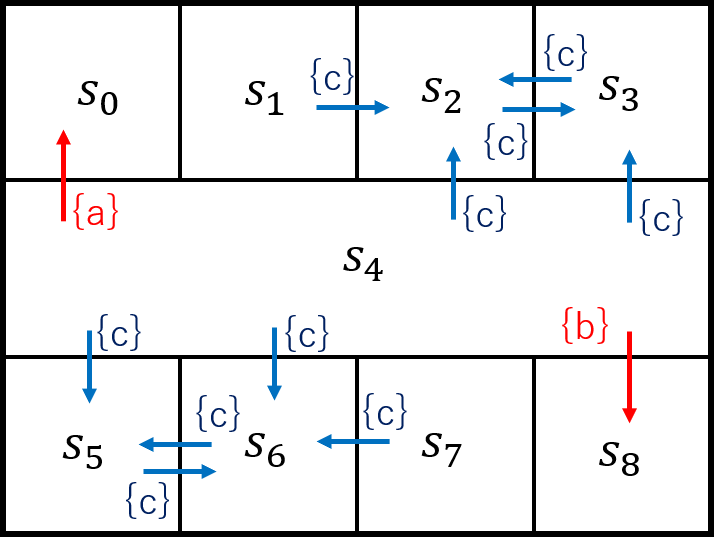
\includegraphics[bb=0 0 377 290,height=3.5cm,width=5cm]{MDP_corridor.png}
%    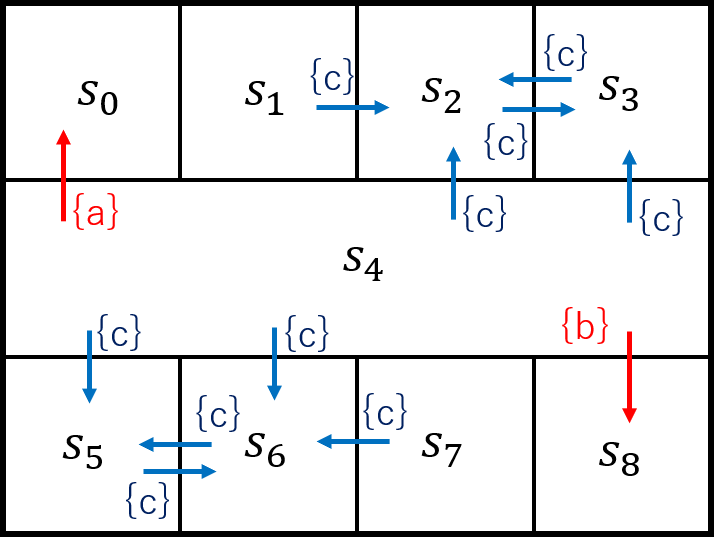
\includegraphics[height=4cm, width=6cm]{MDP_corridor.png}
    \caption{The environment consisting of eight rooms and one corridor. Red arcs are the transitions that we want to occur infinitely often, while blue arcs are the transitions that we never want to occur. $s_7$ is the initial state.}
    \label{Grid1}
\end{figure}

\begin{figure}[htbp]
   \centering
   \vspace{2mm}
%   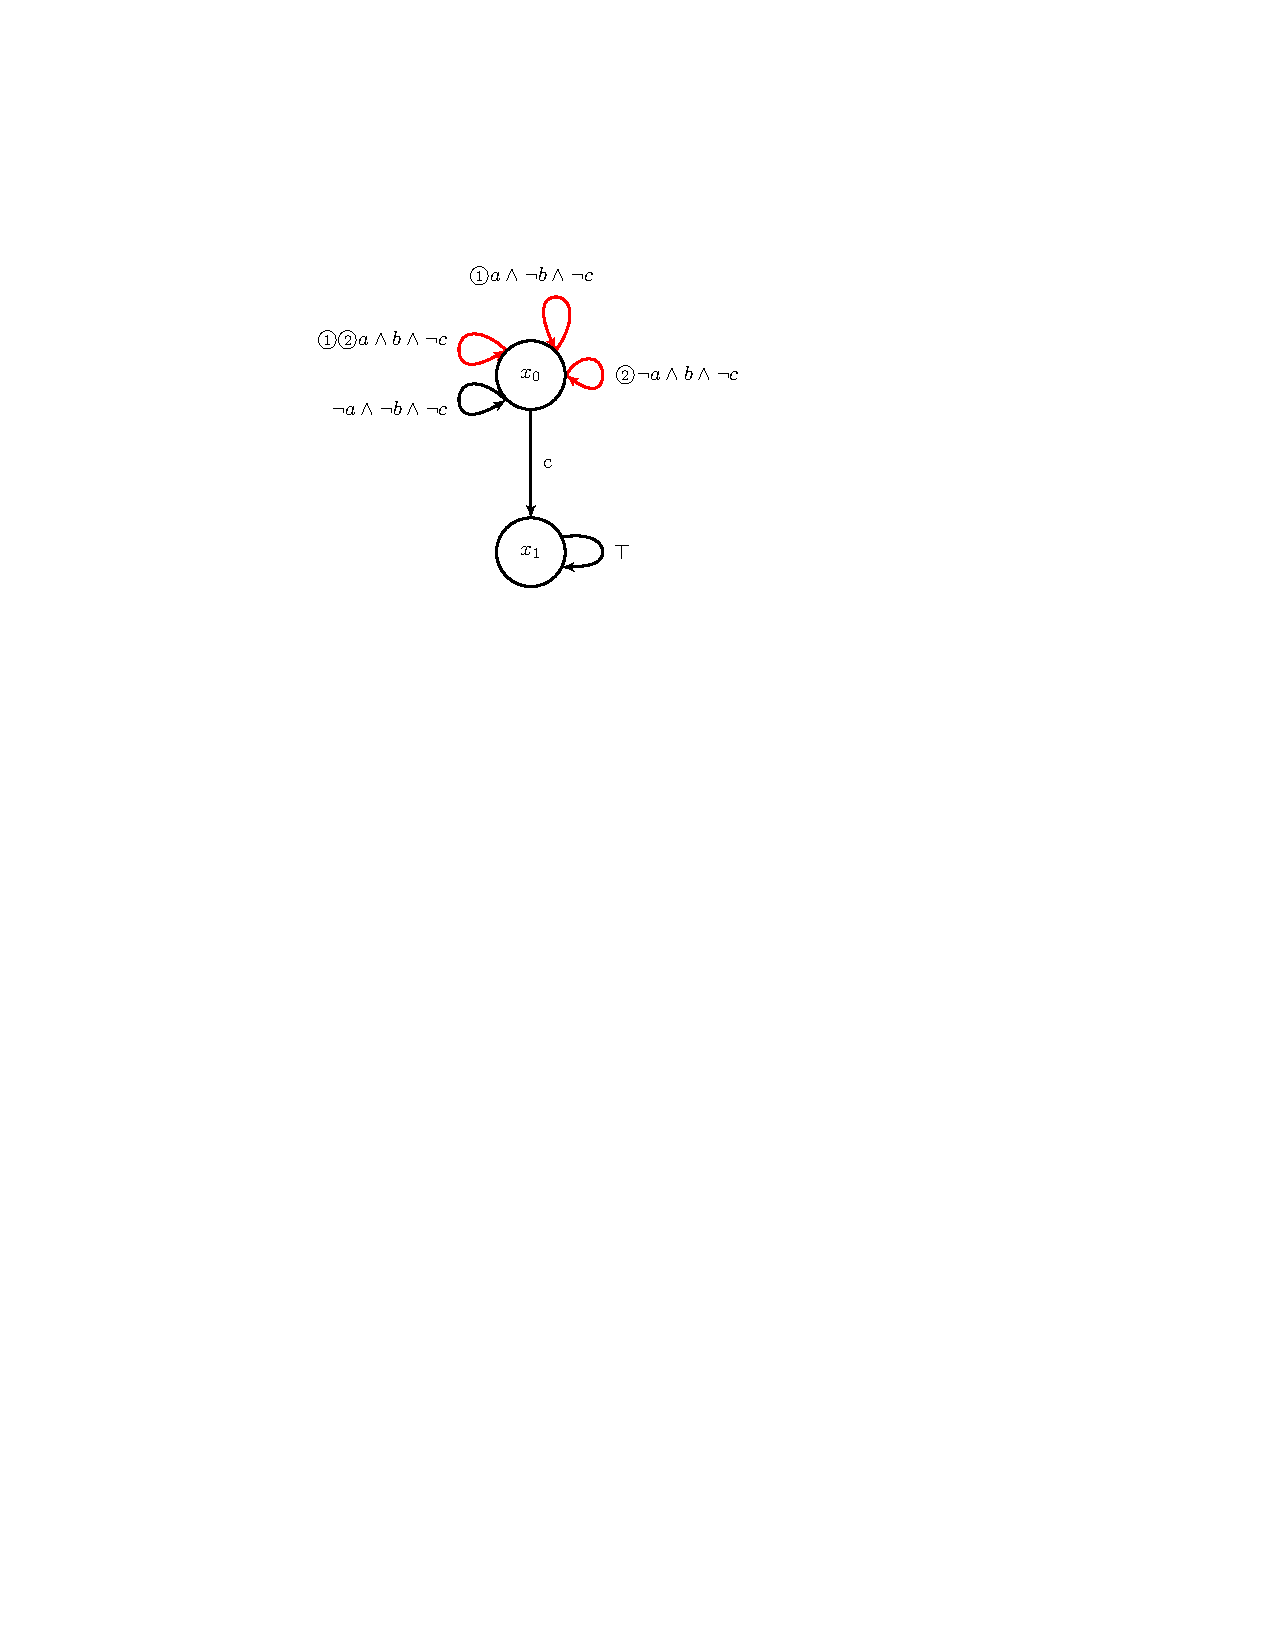
\includegraphics[bb=140 498 368 682,width=5cm]{automaton1.pdf}
   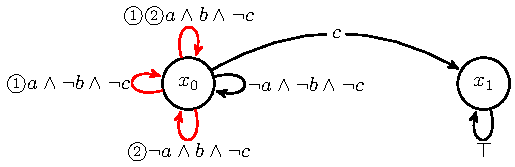
\includegraphics[bb=0 0 247 80,scale=0.65]{ldgba_original.pdf}
   \caption{The tLDBA recognizing the LTL formula $\text{{\bf GF}}a \wedge \text{{\bf GF}}b \wedge \text{{\bf G}}\neg c$, where the initial state is $x_0$. Red arcs are accepting transitions that are numbered in accordance with the accepting sets they belong to, e.g., \textcircled{\scriptsize 1}$a \land \neg b \land \neg c$ means the transition labeled by it belongs to the accepting set $F_1$.}
   \label{automaton}
\end{figure}

\begin{figure}[htbp]
   \centering
%   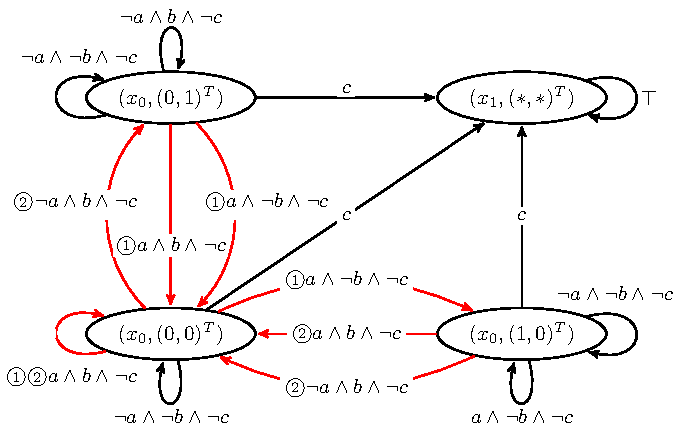
\includegraphics[bb=0 0 374 207,height=4cm, width=7cm]{ldgba.pdf}
   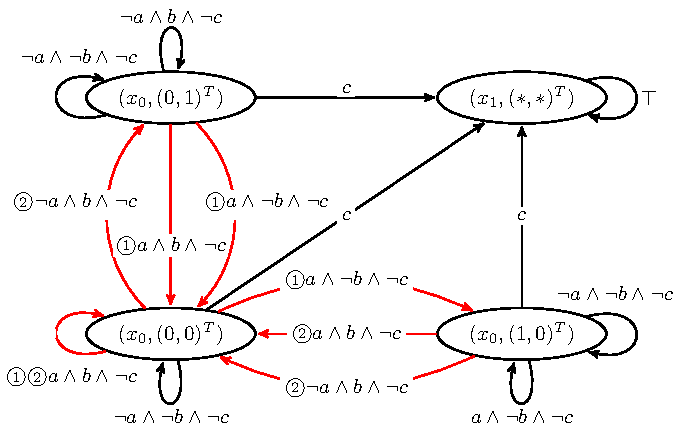
\includegraphics[bb=0 0 374 207,scale=0.6]{ldgba.pdf}
   \caption{The augmented automaton for the tLDBA in Fig.~\ref{automaton} recognizing the LTL formula $\text{{\bf GF}}a \wedge \text{{\bf GF}}b \wedge \text{{\bf G}}\neg c$, where the initial state is $(x_0, (0,0)^T )$. Red arcs are accepting transitions that are numbered in accordance with the accepting sets they belong to. All states corresponding to $x_1$ are merged into $(x_1, (*,*)^T )$.}
   \label{automaton_aug}
\end{figure}

In this section, we evaluate our proposed method and compare it with an existing work.
We consider a path planning problem of a robot in an environment consisting of eight rooms and one corridor as shown in Fig.\ \ref{Grid1}. The state $s_7$ is the initial state and the action space is specified with $\mathcal{A}(s) = \{ Right,\ Left,\ Up,\ Down \}$ for any state $s \neq s_4$ and $\mathcal{A}(s_4) = \{ to\_s_0,\ to\_s_1,\ to\_s_2,$ $\ to\_s_3,\ to\_s_5,\ to\_s_6,\ to\_s_7,\ to\_s_8 \}$, where $to\_s_i$ means attempting to go to the state $s_i$ for $i \in \{0,\ 1,\ 2,\ 3,\ 5,\ 6,\ 7,\ 8 \}$. The robot moves in the intended direction with probability 0.9 and it stays in the same state with probability 0.1 if it is in the state $s_4$. In the states other than $s_4$, it moves in the intended direction with probability 0.9 and it moves in the opposite direction to that it intended to go with probability 0.1. If the robot tries to go to outside the environment, it stays in the same state. The labeling function is as follows.
\begin{align*}
      & L((s, a, s^{\prime})) =
      \left\{
      \begin{aligned}
        & \{ c \} &  & \text{if }s^{\prime} = s_i,\ i \in \{ 2,3,5,6 \}, \nonumber \\
        & \{ a \} &  & \text{if }(s,a,s^{\prime})=(s_4,to\_s_0,s_0), \nonumber \\
        & \{ b \} &  & \text{if }(s,a,s^{\prime})=(s_4,to\_s_8, s_8), \nonumber \\
        & \emptyset &  & \text{otherwise}.
      \end{aligned}
      \right.
    \end{align*}

In the example, the robot tries to take two transitions that we want to occur infinitely often, represented by arcs labeled by \{{\it a}\} and \{{\it b}\}, while avoiding unsafe transitions represented by the arcs labeled by \{{\it c}\}. This is formally specified by the following LTL formula.
\begin{align*}
  \varphi = \text{{\bf GF}}a \wedge \text{{\bf GF}}b \wedge \text{{\bf G}}\neg c.
\end{align*}
The above LTL formula requires the robot to keep on entering the two rooms $s_0$ and $s_8$ from the corridor $s_4$ regardless of the order of entries, while avoiding entering the four rooms $s_2$, $s_3$, $s_5$, and $s_6$.

We use Owl \cite{Owl} to obtain the tLDBA corresponding to the LTL formula.
The tLDBA $B_{\varphi} = (X, x_{init},\Sigma,\delta,\mathcal{F})$ and its augmented automaton $\bar{B}_{\varphi} = (\bar{X},\bar{x}_{init},\bar{\Sigma},\bar{\delta},\bar{\mathcal{F}})$ are shown in Figs.\ \ref{automaton} and \ref{automaton_aug}, respectively. Specifically, the acceptance condition ${\mathcal F}$ of the tLDBA is given by ${\mathcal F} = \{ F_1,F_2 \}$, where $F_1=\{ (x_0, \{ a \}, x_0),\ (x_0, \{ a,b \}, x_0) \}$ and $F_2 = \{ (x_0, \{ b \}, x_0),\ (x_0, \{ a,b \}, x_0) \}$.

We use Q-learning\footnote{We employ Q-learning here but any algorithm that maximizes the discounted expected reward can be applied to our proposed method.} with $\varepsilon$-greedy policy and gradually reduce $\varepsilon$ to 0 to learn an optimal policy asymptotically.
We set the positive reward $r_p = 2$, the epsilon greedy parameter $ \varepsilon = \frac{0.95}{n_t(s^{\otimes})}$, where $n_t(s^{\otimes})$ is the number of visits to state $s^{\otimes}$ within $t$ time steps \cite{Singh1998}, and the discount factor $\gamma = 0.9$. The learning rate $\alpha$ varies in accordance with {\it the Robbins-Monro condition}.

We also evaluate the method in \cite{HAK2019} with the same example.
% They use state-based LDBAs for LTL formulas and construct the product MDP of an MDP and a state-based LDBA to synthesize a policy satisfying the LTL formula. They proposed the accepting frontier function $Acc : X \times 2^X \rightarrow 2^X $ where $X$ is the set of states of the state-based LDBA. Under initializing a set of states $ \mathbb{F} $ with the union of the all accepting sets of the state-based LDBA, the function receives the state $x$ after each transition and the set $\mathbb{F}$. If $x$ is in $\mathbb{F}$, then $Acc$ removes the accepting sets containing $x$ from $\mathbb{F}$. The reward function is based on the varying set $\mathbb{F}$.
We conduct the same example with their method using the tLDBA instead and the same reward value.

Figs.\ \ref{result} and \ref{optimal} show the average reward and the optimal policy, respectively, as a result of the learning when using our proposed method and the method in \cite{HAK2019} after 10000 iterations and 1000 episodes. The arithmetic mean of average reward in each episode for 20 learning sessions is displayed per 100 episodes in Fig.\ \ref{result}.

The results suggest that our proposed method can synthesize a policy satisfying $\varphi$ on the MDP, while the method in \cite{HAK2019} cannot. This is because it is impossible that the transitions labeled by $\{ a \}$ and $\{ b \}$ occur from $s_4$ infinitely often by any positional policy with the tLDBA. In detail, the state of the tLDBA is always $x_0$ while the agent does not move to states $s_2$, $s_3$, $s_5$, and $s_6$. Thus, the state of the product MDP is always $(s_4, x_0)$ while the agent stays in $s_4$. Therefore, the method in \cite{HAK2019} may not synthesize policies satisfying LTL specifications depending on the setting of MDPs or LTL specifications.

\begin{figure}[tbp]
 \centering
 \begin{tabular}{c}
  \begin{minipage}{0.5\hsize}
     \centering
%     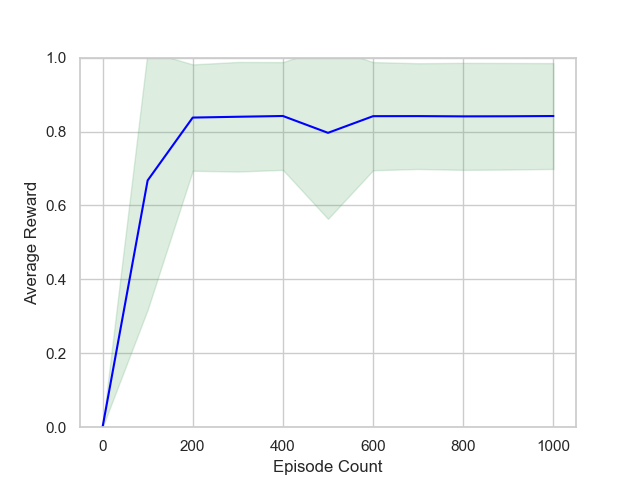
\includegraphics[width=4.5cm]{ep_1000_it_10000_MDP3_gamma_095_re2_ini22_nts_c095_20times.png}
     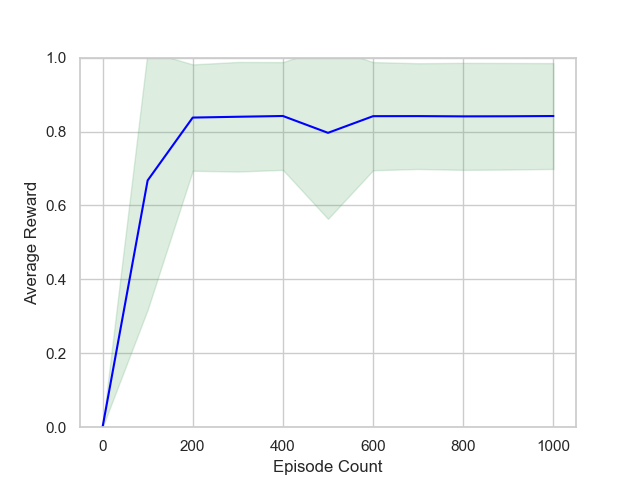
\includegraphics[bb=0 0 461 346, height = 3.4cm, width=4.2cm]{ep_1000_it_10000_MDP3_gamma_095_re2_ini22_nts_c095_20times.png}
 \end{minipage}

 \begin{minipage}{0.5\hsize}
   \centering
%   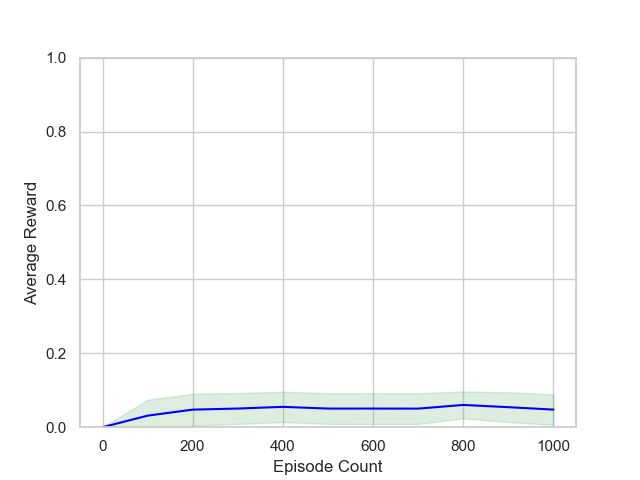
\includegraphics[width=4.5cm]{ep_1000_it_10000_MDP3_gamma_095_nts_c095_abate_20times.png}
   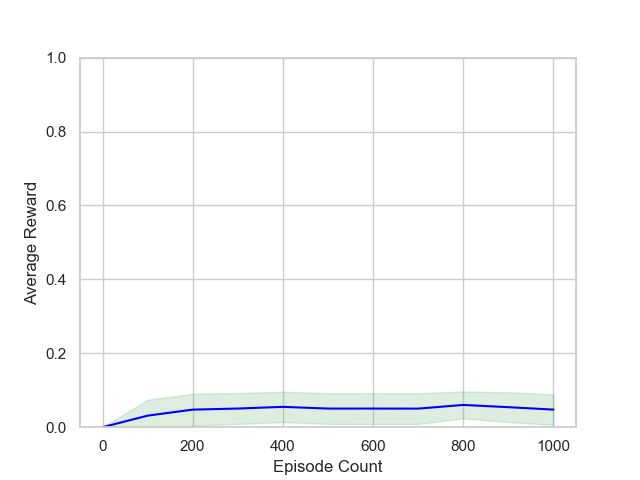
\includegraphics[bb=0 0 461 346, height = 3.4cm, width=4.2cm]{ep_1000_it_10000_MDP3_gamma_095_nts_c095_abate_20times.png}
 \end{minipage}
\end{tabular}
 \caption{The arithmetic mean of average reward in each episode for 20 learning sessions obtained from our proposed method (left) and the method by Hasanbeig $et\ al.$\cite{HAK2019} (right). They are plotted per 100 episodes and the green areas represent the range of standard deviations.}
 \label{result}
\end{figure}

\begin{figure}[tbp]
	\centering
	\begin{tabular}{c}

		\begin{minipage}{0.499\hsize}
			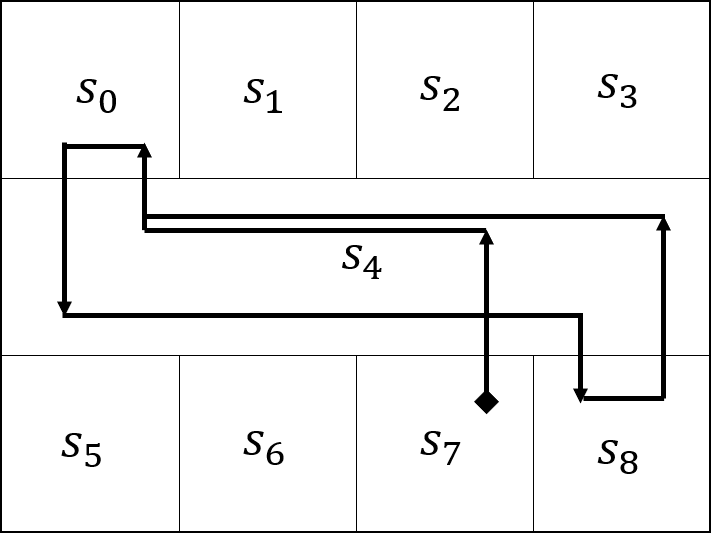
\includegraphics[bb=0 0 341 256, height = 2.8cm, width=3.5cm]{proposed_policy.png}
		\end{minipage}

		\begin{minipage}{0.499\hsize}
			\centering
			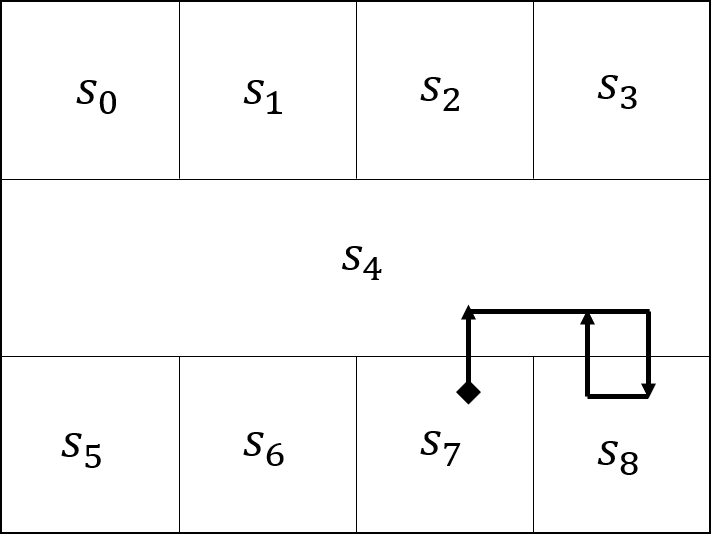
\includegraphics[bb=0 0 341 257, height = 2.8cm, width=3.5cm]{Abate_policy.png}
		\end{minipage}
	\end{tabular}

	\caption{The optimal policy obtained from our proposed method (left) and the method by Hasanbeig $et\ al.$\cite{HAK2019} (right).}
	\label{optimal}
\end{figure}

\section{Conclusions}

The letter proposed a novel RL-based method for the synthesis of a control policy for an LTL specification using a limit-deterministic B\"{u}chi automaton.
The proposed method improved the learning performance compared to an existing method.
It is future work to extend the method to the synthesis of a hierarchical control policy.





%\addtolength{\textheight}{-12cm}   % This command serves to balance the column lengths
                                  % on the last page of the document manually. It shortens
                                  % the textheight of the last page by a suitable amount.
                                  % This command does not take effect until the next page
                                  % so it should come on the page before the last. Make
                                  % sure that you do not shorten the textheight too much.




\begin{thebibliography}{99}
\bibitem{BK2008}
C.\ Baier and J.-P.\ Katoen,
\textit{Principles of Model Checking}.
MIT Press, 2008.
\bibitem{Clarke2018}
E.\ M.\ Clarke, Jr., O.\ Grumberg, D.\ Kroening, D.\ Peled, and H.\ Veith,
\textit{Model Checking}, 2nd Edition.
MIT Press, 2018.
\bibitem{KB2008}
M.\ Kloetzer, C.\ Belta,
``A fully automated framework for control of linear systems from temporal logic specifications,''
\textit{IEEE Trans.\ Autom.\ Contr.}, vol.\ 53, no.\ 1, pp.\ 287--297, 2008.
\bibitem{Gazit2009}
H.\ Kress-Gazit, G.\ E.\ Fainekos, and G.\ J.\ Pappas,
``Temporal-logic-based reactive mission and motion planning,''
\textit{IEEE Trans.\ Robotics}, vol.\ 25, no.\ 6, pp.\ 1370--1381, 2009.
\bibitem{WTM2012a}
T.\ Wongpiromsarn, U.\ Topcu, and R.\ M.\ Murray,
``Receding horizon temporal logic planning,''
\textit{IEEE Trans.\ Autom.\ Contr.}, vol.\ 57, no.\ 11, pp.\ 2817--2830, 2012.
\bibitem{SU2018}
A.\ Sakakibara and T.\ Ushio,
``Decentralized supervision and coordination of concurrent discrete event systems under LTL constraints,''
 in \textit{Proc.\ 14th International Workshop on Discrete Event Systems}, 2018, pp.\ 18-23.
\bibitem{Belta2017}
C.\ Belta, B.\ Yordanov, and E.\ A.\ Gol,
\textit{Formal Methods for Discrete-Time Dynamical Systems}.
Springer, 2017.
\bibitem{Puterman}
M.\ L.\ Puterman,
\textit{Markov Decison Processes, Discrete Stochastic Dynamic Programming}.
John Wiley \& Sons, Inc., 1994.

\bibitem{WTM2012}
E.\ M.\ Wolff, U.\ Topcu, and R.\ M.\ Murray,
``Robust control of uncertain Markov decision processes with temporal logic specifications,''
in \textit{Proc.\ 51st IEEE Conference on Decision and Control}, 2012, pp.\ 3372--3379.
\bibitem{Sadigh2014}
D.\ Sadigh, E.\ S.\ Kim, A.\ Coogan, S.\ S.\ Sastry, and S.\ Seshia,
``A learning based approach to control synthesis of Markov decision processes for linear temporal logic specifications,''
\textit{in Proc.\ 53rd IEEE Conference on Decision and Control}, pp.\ 1091-1096, 2014.
\bibitem{Sutton}
R.\ S.\ Sutton and A.\ G.\ Barto,
\textit{Reinforcement Learning: An Introduction}, 2nd Edition.
MIT Press, 2018.
\bibitem{HU2015}
M.\ Hiromoto and T.\ Ushio,
``Learning an optimal control policy for a Markov decision process under linear temporal logic specifications,''
in \textit{Proc.\ 2015 IEEE Symposium on Adaptive Dynamic Programming and Reinforcement Learning}, 2015, pp.\ 548-555.
\bibitem{SEJK2016}
S.\ Sickert, J.\ Esparaza, S.\ Jaax, and J.\ K\v{r}et\`{i}nsk\'{y},
``Limit-deterministic B\"{u}chi automata for linear temporal logic,''
 in \textit{International Conference on Computer Aided Verification}, 2016, pp.\ 312-332.
\bibitem{HAK2019}
M.\ Hasanbeig, A.\ Abate, and D.\ Kroening,
``Logically-constrained reinforcement learning,'' \textit{arXiv:1801.08099v8}, Feb.\ 2019.
\bibitem{Hahn2019}
E.\ M.\ Hahn, M.\ Perez, S.\ Schewe, F.\ Somenzi, A.\ Triverdi, and D.\ Wojtczak,
``Omega-regular objective in model-free reinforcement learning,''
\textit{Lecture Notes in Computer Science}, no.\ 11427, pp.\ 395--412, 2019.
\bibitem{HKAKPL2019}
M.\ Hasanbeig, Y.\ Kantaros, A.\ Abate, D.\ Kroening, G.\ J.\ Pappas, and I.\ Lee,
``Reinforcement learning for temporal logic control synthesis with probabilistic satisfaction guarantee,''
\textit{arXiv:1909.05304v1}, 2019.
\bibitem{BWZP2019}
A.\ K.\ Bozkurt, Y.\ Wang, M.\ Zavlanos, and M.\ Pajic,
``Control synthesis from linear temporal logic specifications using model-free reinforcement learning,''
\textit{arXiv:1909.07299}, 2019.
\bibitem{ESS}
R.\ Durrett,
\textit{Essentials of Stochastic Processes}, 2nd Edition. ser. Springer texts in statistics. New York; London; Springer, 2012.
\bibitem{ISP}
L.\ Breuer,
``Introduction to Stochastic Processes,'' [Online]. Available: https://www.kent.ac.uk/smsas/personal/lb209/files/sp07.pdf
\bibitem{SM}
S.M.\ Ross,
\textit{Stochastic Processes}, 2nd Edition. University of California, Wiley, 1995.
\bibitem{Singh1998}
S. Singh, T. Jaakkola, M. L. Littman, and C. Szepes\'{v}ari,
``Convergence results for single-step on-policy reinforcement learning algorithms'' \textit{Machine Learning},
vol.~38, no.~3, pp,~287--308, 1998.
\bibitem{Owl}
J.~Kretínsk\'{y}, T.~Meggendorfer, S.~Sickert, ``Owl: A library for $\omega$-words, automata,
and LTL,'' in \textit{Proc.~16th International Symposium on Automated Technology for Verification and Analysis}, 2018,  pp.~543–550.
%https://doi.org/10.1007/978-3-030-01090-4\_34

\end{thebibliography}


\end{document}
